\section{Esercitazione 1}
\title{LEZIONE 8 23/03/2020}\newline
\textbf{link} \href{https://onedrive.live.com/?authkey=%21AATVJK3srNwxGzs&id=EE092FF4FF7B5B0E%212158&cid=EE092FF4FF7B5B0E}{clicca qui per una registrazione di back up}\newline
\newline
Appunti del prof con annotazioni \url{../pdf/FdA-L08-2020.03.23.pdf}\newline
Contenuto:
\begin{itemize}
    \item Calcolo del movimento con formule di Laplace e con la trasformata di Laplace;
    \item esponenziale di matrice;
    \item Stabilità con matrice $A$ non diagonalizzabile;
    \item Funzione di trasferimento;
    \item Schema a blocchi (stesura dello schema a blocchi con integratore e senza);
    \item Calcolo del movimento libero con autovalori complessi;
\end{itemize}
\subsection{Schema a blocchi}
\subsubsection{Primo metodo (analitico)}
\begin{itemize}
    \item Si trasforma il sistema $\begin{cases}
        \dot{x} = A x + bu\\ y = cx +d
    \end{cases}$ secondo Laplace: $\begin{cases}
        s X = A X + b U\\ Y = c X + d
    \end{cases}$;
    \item Si esprime il sistema secondo le variabili di stato e secondo l'uscita:$\begin{cases}
        X = \;\text{qualcosa}\;\\ Y = \;\text{qualcosa}\;
    \end{cases}$;
    \item Ora è facile ricostruire lo schema a blocchi.
\end{itemize}
\subsubsection{Secondo metodo (Funzione di trasferimento)}
\begin{itemize}
    \item Si calcola la funzione di trasferimento $G(s)$;
    \item Ricordando che $Y = G(s) U$ possiamo scrivere il sistema a blocchi come: $Y \longrightarrow \left[G(s)\right] \longrightarrow U$
\end{itemize}
\subsubsection{Terzo metodo (Integratori)}
Ricordiamo che la funzione integrale nel dominio delle trasformate è rappresentato dall'aggiunta di un termine $\frac{1}{s}$ (\textbf{es.} $y(t) = \int_{0}^{t}u(\tau)d \tau \Rightarrow Y(s) = \frac{1}{s} U(s)$ ).\newline
Il termine $\frac{1}{s}$ è la funzione di trasferimento dell'integratore.
\begin{itemize}
    \item Si disegnano $n$ blocchi integratori $\frac{1}{s}$ quante sono le $n$ variabili di stato del sistema;
    \item Per ciascuno di questi blocchi $n$ si mette come ingresso la variabile derivata ($\dot{x}_n$) e come uscita la variabile semplice ($x_n$);
    \item Osservando le matrici $A$ e $b$ si compongono con dei nodi sommatori i vari $\dot{x}_1, \dots, \dot{x}_n$;
    \item Infine osservando le matrici $c$ e $d$ si compone l'uscita.
\end{itemize}
[immagine dagli appunti del prof]
\begin{center}
    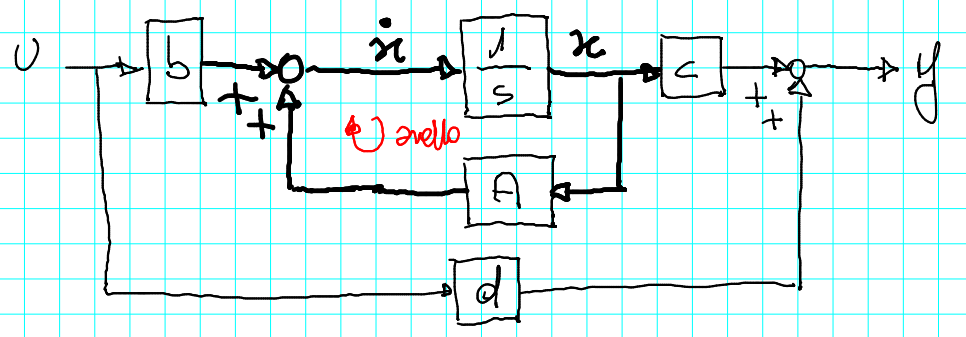
\includegraphics[height=3cm]{../lezione8/img1.PNG}
\end{center}
Rappresentazioen di dove solitamente si inseriscono i valori delle matrici del sistema all'interno dello schema a blocchi sviluppato con l'integratore.
